



\documentclass[first=dgreen,second=purple,logo=yellowexc]{aaltoslides}
%\documentclass{aaltoslides} % DEFAULT
%\documentclass[first=purple,second=lgreen,logo=redque,normaltitle,nofoot]{aaltoslides} % SOME OPTION EXAMPLES





% input encode
\usepackage[utf8]{inputenc}


%\usepackage[T1]{fontenc}
%\usepackage{lastpage}
%\usepackage{multirow}
%\usepackage{colortbl}
%\usepackage{comment}
%\usepackage{bm}
%\usepackage{natbib}


% Lipsum package generates bullshit
%\usepackage{lipsum}

% Set the document languages
%\usepackage[finnish,swedish,english]{babel}

% nomenclature
%\usepackage[intoc]{nomencl}

% math
\usepackage{amsmath}

% bibliograph
%\usepackage{natbib}

% For algorithms
\usepackage{algorithm}
\usepackage{algorithmic}

% math font
\usepackage{amsfonts}

% theory
%\usepackage{amsthm}

% double bracket
\usepackage{stmaryrd}

% special math symbol
\usepackage{amssymb}

% use enumerate environment
%\usepackage{enumitem}

% use \url \hyperref, make reference clickable
\usepackage{hyperref}

% use lastpage to inde
\usepackage{lastpage}



%-------------------
%
% set
%
%-------------------
\newcommand{\Acal}{\mathcal{A}}
\newcommand{\Bcal}{\mathcal{B}}
\newcommand{\Ccal}{\mathcal{C}}
\newcommand{\Dcal}{\mathcal{D}}
\newcommand{\Ecal}{\mathcal{E}}
\newcommand{\Fcal}{\mathcal{F}}
\newcommand{\Gcal}{\mathcal{G}}
\newcommand{\Hcal}{\mathcal{H}}
\newcommand{\Ical}{\mathcal{I}}
\newcommand{\Jcal}{\mathcal{J}}
\newcommand{\Kcal}{\mathcal{K}}
\newcommand{\Lcal}{\mathcal{L}}
\newcommand{\Mcal}{\mathcal{M}}
\newcommand{\Ncal}{\mathcal{N}}
\newcommand{\Ocal}{\mathcal{O}}
\newcommand{\Pcal}{\mathcal{P}}
\newcommand{\Qcal}{\mathcal{Q}}
\newcommand{\Rcal}{\mathcal{R}}
\newcommand{\Scal}{\mathcal{S}}
\newcommand{\Tcal}{\mathcal{T}}
\newcommand{\Ucal}{\mathcal{U}}
\newcommand{\Vcal}{\mathcal{V}}
\newcommand{\Wcal}{\mathcal{W}}
\newcommand{\Xcal}{\mathcal{X}}
\newcommand{\Ycal}{\mathcal{Y}}
\newcommand{\Zcal}{\mathcal{Z}}

\newcommand{\RR}{\mathbb{R}}
\newcommand{\ZZ}{\mathbb{Z}}

%-------------------
%
% vector
%
%-------------------
\newcommand{\va}{\mathbf {a}}
\newcommand{\vb}{\mathbf {b}}
\newcommand{\vc}{\mathbf {c}}
\newcommand{\vd}{\mathbf {d}}
\newcommand{\ve}{\mathbf {e}}
\newcommand{\vf}{\mathbf {f}}
\newcommand{\vg}{\mathbf {g}}
\newcommand{\vh}{\mathbf {h}}
\newcommand{\vi}{\mathbf {i}}
\newcommand{\vj}{\mathbf {j}}
\newcommand{\vk}{\mathbf {k}}
\newcommand{\vl}{\mathbf {l}}
\newcommand{\vm}{\mathbf {m}}
\newcommand{\vn}{\mathbf {n}}
\newcommand{\vo}{\mathbf {o}}
\newcommand{\vp}{\mathbf {p}}
\newcommand{\vq}{\mathbf {q}}
\newcommand{\vr}{\mathbf {r}}
\newcommand{\vs}{\mathbf {s}}
\newcommand{\vt}{\mathbf {t}}
\newcommand{\vu}{\mathbf {u}}
\newcommand{\vv}{\mathbf {v}}
\newcommand{\vw}{\mathbf {w}}
\newcommand{\vx}{\mathbf {x}}
\newcommand{\vy}{\mathbf {y}}
\newcommand{\vz}{\mathbf {z}}
\newcommand{\vmu}{\mathbf {\mu}}
\newcommand{\valpha}{\mathbf {\alpha}}
\newcommand{\vlambda}{\mathbf {\lambda}}
\newcommand{\vAlpha}{\mathbf {\Alpha}}
\newcommand{\vbeta}{\mathbf {\beta}}
\newcommand{\vBeta}{\mathbf {\Beta}}
\newcommand{\vgamma}{\mathbf {\gamma}}
\newcommand{\vGamma}{\mathbf {\Gamma}}
\newcommand{\vdelta}{\mathbf {\dalta}}
\newcommand{\vDelta}{\mathbf {\Dalta}}
\newcommand{\vone}{\mathbf {1}}
\newcommand{\vzero}{\mathbf {0}}
\newcommand{\vell}{\mathbf {\ell}}
\newcommand{\vxi}{\mathbf{\xi}}
\newcommand{\vphi}{\mathbf{\phi}}
\newcommand{\vPhi}{\mathbf{\Phi}}

%-------------------
%
% math operation
%
%-------------------
\newcommand{\argmax}{\textbf{argmax}}
\newcommand{\argmin}{\textbf{argmin}}
\newcommand{\sign}{\textbf{sign}}
\newcommand{\maximize}{\textbf{max}}
\newcommand{\minimize}{\textbf{min}}
\newcommand{\argkmax}{\textbf{argkmax}}
\newcommand{\argkmin}{\textbf{argkmin}}
\newcommand{\kmaximize}{\textbf{kmax}}
\newcommand{\kminimize}{\textbf{kmin}}
\newcommand{\st}{\textbf{s.t.}}
\newcommand{\set}[1]{\{ #1 \}}
%\newcommand{\ind}[1]{{\llbracket #1 \rrbracket}}
\newcommand{\ind}[1]{\mathbf{1}_{\{#1\}}}
\newcommand{\norm}[1]{\left|\left| #1 \right|\right|}
\newcommand{\ip}[2]{\langle #1, #2 \rangle}
\newcommand{\var}{\textbf{Var}}
\newcommand{\E}{\textbf{E}}
\newcommand{\exponential}[1]{e^{ #1 }}


\newcommand{\Gva}{G_{\va}}
%-------------------
%
% writings
%
%-------------------
\newcommand{\eqdef}{\overset{{\rm \mbox{\tiny def}}}{=}}
\newcommand{\sbf}[1]{\boldsymbol{#1}}
\newcommand{\mbf}[1]{\mathbf{#1}} 
\newcommand{\etal}{{\em et al.}}

\newcommand{\svmstruct}{{\sc ssvm}}
\newcommand{\mmmn}{{\sc m$^3$n}}
\newcommand{\svm}{{\sc svm}}
\newcommand{\mmcrf}{{\sc mmcrf}}
\newcommand{\smo}{{\sc smo}}
\newcommand{\crf}{{\sc crf}}
\newcommand{\nphard}{$\Ncal\Pcal$-hard}
\newcommand{\nphardness}{$\Ncal\Pcal$-hardness}
\newcommand{\iis}{{\sc iis}}
\newcommand{\memm}{{\sc memm}}
\newcommand{\lr}{{\sc lr}}
\newcommand{\svmlight}{{\sc svmlight}}
\newcommand{\libsvm}{{\sc libsvm}}
\newcommand{\svmcascade}{{\sc svmcascade}}
\newcommand{\adaboost}{{\sc adaboost}}
\newcommand{\adaboostmh}{{\sc adaboost.mh}}
\newcommand{\bagging}{{\sc bagging}}
\newcommand{\vrtree}{{\sc vr-tree}}
\newcommand{\deepboosting}{{\sc deepboosting}}
\newcommand{\loo}{{\sc loo}}
\newcommand{\mtl}{{\sc mtl}}
\newcommand{\sdp}{{\sc sdp}}
\newcommand{\iqp}{{\sc iqp}}
\newcommand{\qp}{{\sc qp}}
\newcommand{\daggraph}{{\sc dag}}
\newcommand{\lp}{{\sc lp}}

\newcommand{\hatf}{{\hat{f}}}
\newcommand{\p}{\sc p}
\newcommand{\n}{\sc n}
\newcommand{\pp}{\sc pp}
\newcommand{\pn}{\sc pn}
\newcommand{\nn}{\sc nn}
\newcommand{\maxcut}{{\sc max-cut}}
\newcommand{\greedy}{{\sc greedy}}
\newcommand{\kernelcascade}{{\sc kernel cascade}}
\newcommand{\netrate}{{\sc netrate}}
\newcommand{\netinf}{{\sc netinf}}
\newcommand{\spin}{{\sc spin}}
\newcommand{\vI}{\mathbf{I}}
\newcommand{\tp}{^{\intercal}}
\newcommand{\mve}{{\sc mve}}
\newcommand{\amm}{{\sc amm}}
\newcommand{\mam}{{\sc mam}}
\newcommand{\rta}{{\sc rta}}
\newcommand{\lasso}{{\sc lasso}}
\newcommand{\mle}{{\sc mle}}
\newcommand{\map}{{\sc map}}
\newcommand{\rbf}{{\sc rbf}}
\newcommand{\mlknn}{{\sc ml-knn}}
\newcommand{\knn}{{\sc knn}}
\newcommand{\iblr}{{\sc iblr}}
\newcommand{\cc}{{\sc cc}}
\newcommand{\pcc}{{\sc pcc}}
\newcommand{\ecc}{{\sc ecc}}
\newcommand{\br}{{\sc br}}
\newcommand{\corrlog}{{\sc corrlog}}
\newcommand{\ilgs}{{\sc ilgs}}
\newcommand{\ilrs}{{\sc ilrs}}
\newcommand{\cpp}{{\sc c}}
\newcommand{\matlab}{{\sc matlab}}
\newcommand{\openmp}{{\sc openmp}}
\newcommand{\python}{{\sc python}}
\newcommand{\cvx}{{\sc cvx}}
\newcommand{\lda}{{\sc lda}}
\newcommand{\kkt}{{\sc k.k.t}}
\newcommand{\lbp}{{\sc lbp}}
\newcommand{\anova}{{\sc anova}}

\renewcommand{\algorithmicrequire}{\textbf{Input:}}
\renewcommand{\algorithmicensure}{\textbf{Output:}}



\newcommand{\Upsilonb}{\pmb \Upsilon}
\newcommand{\phib}{\pmb \phi}
\newcommand{\psib}{\pmb \psi}
\newcommand{\varphib}{\pmb \varphi}
\newcommand{\phibh}{\hat\phib}
\newcommand{\psibh}{\hat \psib}
\newcommand{\vYcal}{\pmb \Ycal}
\newcommand{\vXcal}{\pmb \Xcal}
\newcommand{\vFcal}{\pmb \Fcal}
%-------------------
%
% others
%
%-------------------




%\newtheorem{definition}{Definition}
%\newtheorem{theory}{Theory}
%\newtheorem{lemma}{Lemma}

















\title{Structured output prediction for multilabel classification}
\author{Hongyu Su}



\institute[ICS]{
Helsinki Institute for Information Technology HIIT\\
Department of Computer Science, Aalto University
}

\aaltofootertext{Structured output prediction}{\today}{\arabic{page}\ }


\date{ \today} %\date{Version 1.0, \today}

\iffalse
\AtBeginSection[]
{
  \begin{frame}<beamer>{Outline}
    \tableofcontents[currentsection,subsection]
  \end{frame}
}
\fi




%--------------------------------
%
% document
%
%--------------------------------

\begin{document}

\aaltotitleframe
\footnotesize

%
\begin{frame}{Multilabel classification}
	\begin{itemize}\footnotesize
		\item {\em Multilabel classification} is an important research field in machine learning.
		\item Input variable $\vx\in\vXcal$ is in $d$ dimensional input space $\vXcal=\RR^d$.
		\item Output variable $\vy=(y_1,\cdots,y_l)\in\vYcal$ is a binary vector consist of $l$ binary variables $y_j\in\{+1,-1\}$.
		\item $\vy$ is called a multilabel, $y_j$ is called a microlabel.
		\item Output space is composed by a Cartesian product of $l$ sets
		\begin{align*}
			\vYcal=\Ycal_1\times\cdots\times\Ycal_l,\,\Ycal_i=\{+1,-1\}.
		\end{align*}
		\item For example, in document classification, a document $\vx$ can be classified as ``news'', ``movie'', and ``science''
		\begin{align*}
\vy=(\underbrace{+1}_{\text{news}},\underbrace{+1}_{\text{movie}},\underbrace{-1}_{\text{sports}},\underbrace{-1}_{\text{politics}},\underbrace{-1}_{\text{finance}},\underbrace{+1}_{\text{science}},\underbrace{-1}_{\text{art}}).
		\end{align*}\footnotesize
		\item The goal is to find a mapping function $f\in\Hcal$ that predicts the best values of an output given an input $f:\vXcal\rightarrow\vYcal$.
	\end{itemize}
\end{frame}

%
\begin{frame}{Central problems in multilabel classification}
	\begin{itemize}\footnotesize
		\item The size of the output space (searching space) is exponential in the number of microlabels.
		\begin{align*}
			\vYcal=\Ycal_1\times\cdots\times\Ycal_l,\,\Ycal_i=\{+1,-1\}\quad|\vYcal| = 2^l.
		\end{align*}
		\item The dependency of microlabels needs to be exploited to improve the prediction performance.
		\begin{itemize}\footnotesize
			\item If a document is about ``movie'', then it is more likely to be about ``art'' than ``science''.
		\end{itemize}
	\end{itemize}
\end{frame}

%
\begin{frame}{Real world applications}
	\begin{itemize}\footnotesize
		\item Social network, information can spread through multiple users. 
		\begin{tabular}{p{3cm}p{10cm}} 
	    \multirow{2}{*}{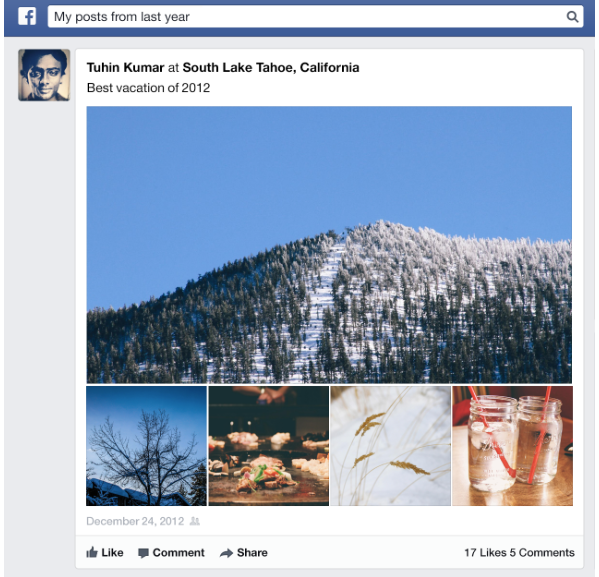
\includegraphics[scale = 0.06]{./figures/facebookvideo.png}} & \\
		& $\vy=(\underbrace{+1}_{\text{Ted}},\underbrace{-1}_{\text{Alice}},\underbrace{+1}_{\text{David}},\underbrace{-1}_{\text{Mark}},\underbrace{+1}_{\text{Alex}},\underbrace{-1}_{\text{Zoe}},\underbrace{-1}_{\text{Frank}})$\\
	    \end{tabular}
		\item Image annotation, an image can associate with multiple tags.
		\begin{tabular}{p{3cm}p{10cm}}
        \multirow{2}{*}{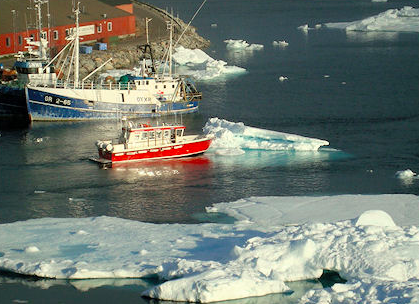
\includegraphics[scale = 0.11]{./figures/boatsea.png}} & \\
		& $\vy=(\underbrace{+1}_{\text{boat}},\underbrace{+1}_{\text{sea}},\underbrace{-1}_{\text{sun}},\underbrace{-1}_{\text{beach}},\underbrace{-1}_{\text{people}},\underbrace{+1}_{\text{ice}},\underbrace{+1}_{\text{land}})$\\
        \end{tabular}
		\item Document classification, an article can be assigned to multiple categories.
		\begin{tabular}{p{3cm}p{10cm}} 
        \multirow{2}{*}{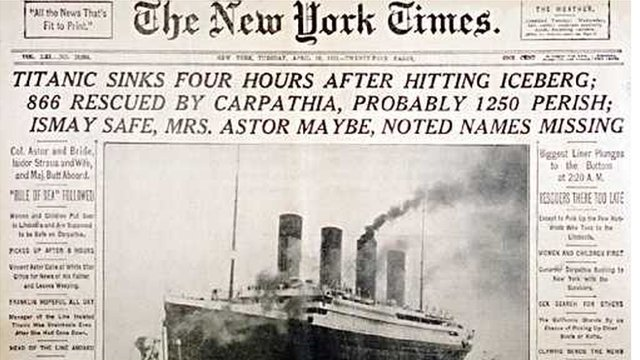
\includegraphics[scale = 0.11]{./figures/titanic.jpg}} & \\
		& $\vy=(\underbrace{+1}_{\text{news}},\underbrace{+1}_{\text{economics}},\underbrace{-1}_{\text{sports}},\underbrace{-1}_{\text{politics}},\underbrace{-1}_{\text{movie}},\underbrace{-1}_{\text{science}},\underbrace{-1}_{\text{art}})$\\
        \end{tabular}
		\item Drug discovery, a drug can be effective for multiple symptoms.
		\begin{tabular}{p{3cm}p{10cm}} 
        \multirow{2}{*}{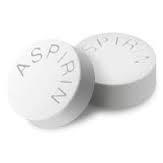
\includegraphics[scale = 0.25]{./figures/aspirin.jpg}} & \\
		& $\vy=(\underbrace{+1}_{\text{heart}},\underbrace{+1}_{\text{stroke}},\underbrace{+1}_{\text{blood}},\underbrace{+1}_{\text{fever}},\underbrace{-1}_{\text{digest}},\underbrace{-1}_{\text{liver}},\underbrace{+1}_{\text{swelling}})$\\
        \end{tabular}
	\end{itemize}
\end{frame}

%
\begin{frame}{Flat multilabel classification approaches}
	\begin{itemize}\footnotesize
		\item The categorization is proposed in \cite{Tsoumakas10mining}
		\item Problem transformation
		\begin{itemize}\footnotesize
			\item Model the multilabel classification as a collection of single-label classification problems and solve each problem independently.
			\item For example, \mlknn\ \cite{Zhang07mlknn}, \cc\ \cite{Read09classifier,Read11classifier}, \iblr\ \cite{Cheng09combining}.
		\end{itemize}
		\item Algorithm adaptation 
		\begin{itemize}\footnotesize
			\item Modify the single-label classification algorithm for multilabel classification problems.
			\item For example, \adaboostmh\ \cite{Schapire99improved,Esuli2008boosting}, \corrlog\ \cite{Bian12corrlog}, \mtl\ \cite{Argyriou08convex}.
		\end{itemize}
		\item These approaches does not model the dependency structure explicitly.
	\end{itemize}
\end{frame}

%
\begin{frame}{Structured output prediction}
	\begin{itemize}\footnotesize
		\item Model the dependency structure with an output graph defined on microlabels.
		\item The categorization is proposed in \cite{Su2014Multilabel}.
		\item Hierarchical classification
		\begin{itemize}\footnotesize
			\item The output graph is a rooted tree or a \daggraph\ defining different levels of granularities.
			\item For example, \svmstruct\ \cite{THJA04,TJTA05}.
		\end{itemize}
		\item Graph labeling
		\begin{itemize}\footnotesize
			\item The output graph takes a more general form (e.g., a tree, a chain).
			\item For example, \crf\ \cite{lafferty01,taskar02}, \mmmn\ \cite{Taskar04max}, \mmcrf\ \cite{Rousu07, su10structured}, \spin\ \cite{su14structured}.
		\end{itemize}
		\item These approaches assume the output graph is known {\em apriori}.
	\end{itemize}
\end{frame}

%
\begin{frame}{Contributions}
	\begin{itemize}\footnotesize
		\item Structured output prediction models when the output graph is known.
		\begin{itemize}\footnotesize
			\item \spin\ for network influence prediction \cite{su14structured}.
			\item \mmcrf\ to work with general output graph structures \cite{su10structured}.
		\end{itemize}
		\item Structured output prediction models working with unknown output graph.
		\begin{itemize}\footnotesize
			\item \mve\ to combine multiple structured output predictors with ensemble \cite{su11mutitask}.
			\item \amm\ and \mam\ to aggregate the inference results from multiple structured output predictors \cite{su2013multilabelacml,su15multilabel}.
			\item \rta\ to perform joint learning and inference over a collection of random spanning trees \cite{su14multilabelnips}.
		\end{itemize}
		\item Codes for developed models are available from \href{http://hongyusu.github.io}{http://hongyusu.github.io}.
	\end{itemize}
\end{frame}


%
\begin{frame}{Outline}
	\begin{itemize}\footnotesize
		\item Preliminaries
		\item Structured output learning with known output graph
		\item Structured output learning with unknown output graph
		\item Future work
		\item Experimental results
	\end{itemize}
\end{frame}

%
\begin{frame}{Preliminaries}
	\begin{itemize}\footnotesize
		\item Training examples come in pairs $(\vx,\vy)\in\vXcal\times\vYcal$.
		\item $\vx\in\vXcal$ is an arbitrary input space.
		\item $\vYcal$ is an output space of a collection of $\ell$-dimensional {\em multilabels}.
		\begin{align*}\footnotesize
			\vy=(y_1,\cdots,y_{\ell})\in\vYcal.
		\end{align*}
		\item $y_i$ is a {\em microlabel} and $y_i\in\{1,\cdots,r_i\}, r_i\in\ZZ$.
		\item For example, multilabel binary classification $y_i\in\{-1,+1\}$.
		\item We are given a set of $m$ training examples $\{(\vx_i,\vy_i)\}_{i=1}^m$.
		%\item An arbitrary pair $(\vx_i,\vy),\,\vy_\in\vYcal$ is called pseudo-example.
		\item Each example $(\vx,\vy)$ is mapped into a joint feature space $\phib(\vx,\vy)$.
		\item $\vw$ is the weight vector in the joint feature space.
		\item Define a linear score function $F(\vw,\vx,\vy) = \ip{\vw}{\phib(\vx,\vy)}$.
		\item $\vw$ makes sure example $\vx$ with correct multilabel $\vy$ achieves higher score than with any other incorrect multilabel $\vy'\in\vYcal$.
	\end{itemize}
\end{frame}

\begin{frame}{Inference problem}
	\begin{itemize}
		\item The prediction $\vy_{\vw}(\vx)$ of an input $\vx$ is the multilabel $\vy$ that maximizes the score function 
		\begin{align}\footnotesize
			\vy_{\vw}(\vx) = \underset{\vy\in\vYcal}{\argmax}\,\ip{\vw}{\phib(\vx,\vy)}. \label{inference}
		\end{align}
		\item Search space $|\vYcal|=2^{\ell}$ is exponential in size.
		\item (\ref{inference}) is called {\em inference} problem which is \nphard\ for most output feature maps.
		\item We aim at using an output feature map in which the inference can be solved with a polynomial algorithm, e.g., dynamic programming.
	\end{itemize}
\end{frame}

%
\begin{frame}{Input-output feature maps}
	\begin{itemize}\footnotesize
		\item We assume that the joint feature map $\phib$ is a potential function on a Markov network $G=(E,V)$.
		\item A vertex $v_i\in V$ corresponds to a microlabel $y_i$, an edge $(v_i,v_j)\in E$ corresponds to the pairwise correlation of the microlabel $y_i$ and $y_j$.
		\item $G$ models potential pairwise correlations.
		\begin{center}
			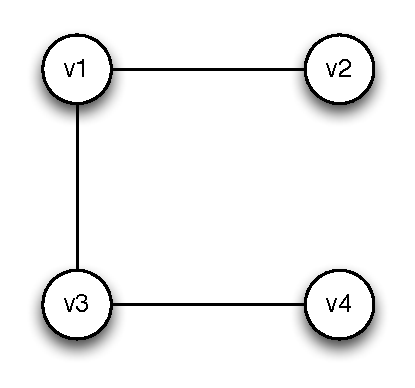
\includegraphics[scale=0.3]{./figures/outputgraph.pdf}
		\end{center}
		\item $\varphib(\vx)\in\RR^d$ is the input feature map, e.g., bag-of-words of a document.
		\item $\psib(\vy)\in\RR^{4|E|}$ is the output feature map which maps the multilabel $\vy$ into a collection of edges and labels
		\begin{align*}\footnotesize
			\varphib(\vy) = (u_{e})_{e\in E},u_e\in\{-1,+1\}^2.
		\end{align*}
	\end{itemize}
\end{frame}

%
\begin{frame}{An example of output feature map}
	\begin{itemize}\footnotesize
		\item Markov network $G=(E,V)$
		\begin{center}
			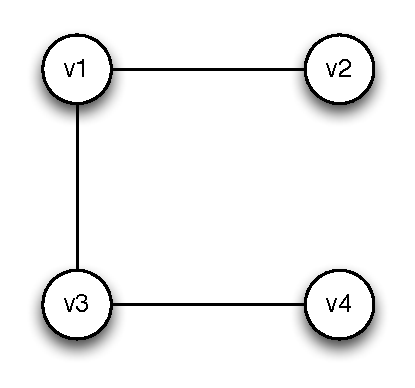
\includegraphics[scale=0.3]{./figures/outputgraph.pdf}
		\end{center}
		\item Multilabel $\vy$
		\begin{align*}
			\vy&=(y_1,y_2,y_3,y_4)=(+1,-1,+1,+1)
		\end{align*}
		\item Output feature map $\psib(\vy)$
		\begin{align*}
			\psib(\vy) &= ( \underbrace{\underbrace{0}_{--}, \underbrace{0}_{-+}, \underbrace{1}_{+-}, \underbrace{0}_{++},}_{(v_1,v_3)} 
			\underbrace{\underbrace{0}_{--}, \underbrace{0}_{-+}, \underbrace{0}_{+-}, \underbrace{1}_{++},}_{(v_1,v_2)}
			\underbrace{\underbrace{0}_{--}, \underbrace{0}_{-+}, \underbrace{0}_{+-}, \underbrace{1}_{++}}_{(v_3,v_4)})
		\end{align*}
	\end{itemize}
\end{frame}

%
\begin{frame}{Joint feature map}
	\begin{itemize}\footnotesize
		\item The joint feature is the Kronecker product of $\varphib(\vx)$ and $\psib(\vy)$
		\begin{align*}\footnotesize
			\phib(\vx,\vy) = (\phib_e(\vx,\vy))_{e\in E}=(\varphib(\vx)\otimes\psib_e(\vy_e))_{e\in E}.
		\end{align*}
		\begin{center}
			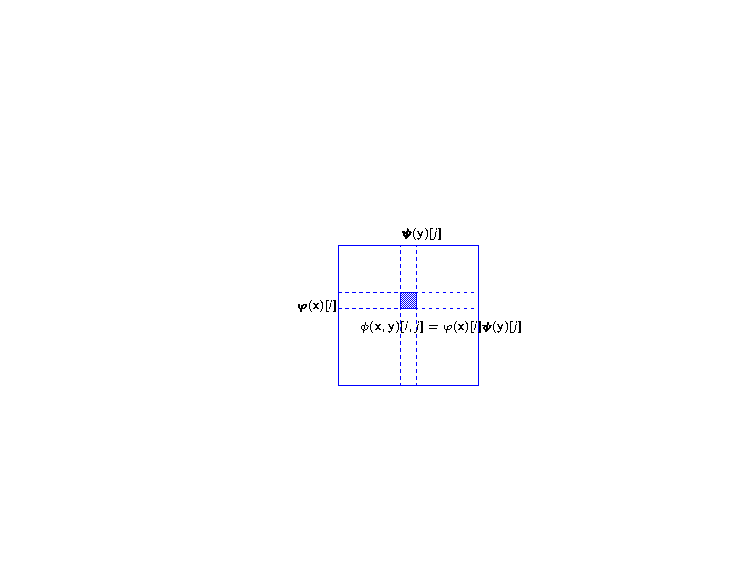
\includegraphics[scale = 1]{./figures/tensor_label.pdf}
		\end{center}
		\item The score function can be factorized by the output graph $G$
		\begin{align*}
			F(\vw,\vx,\vy) = \ip{\vw}{\phib(\vx,\vy)} = \sum_{e\in E}\ip{\vw_e}{\phib_e(\vx,\vy_e)}.
		\end{align*}
	\end{itemize}
\end{frame}

%
\begin{frame}{Optimization problem}
	\begin{itemize}\footnotesize
		\item To learn parameter $\vw$, we aim to maximize the magin between correct pair $(\vx_i,\vy_i)$ and all the other incorrect pairs $(\vx_i,\vy),\vy\in\vYcal/\vy_i$ in the joint feature space $\phib$.
		\begin{center}
			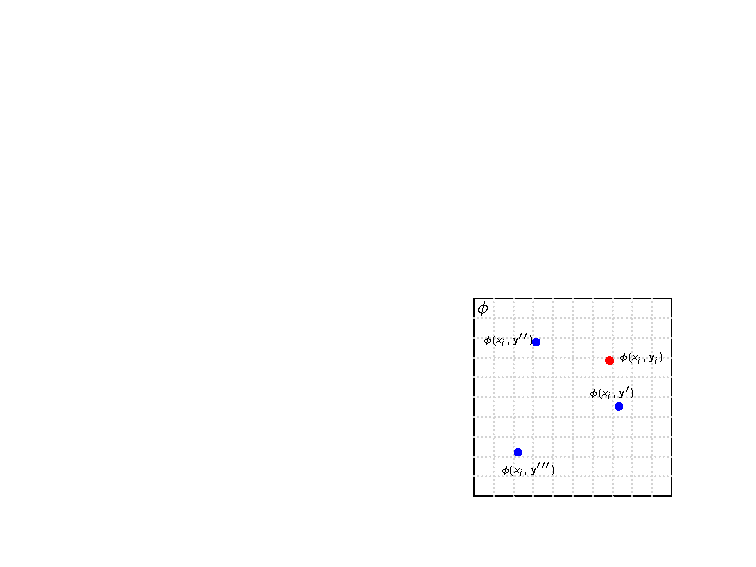
\includegraphics[scale = 0.6]{./figures/jointfeaturespace.pdf}
		\end{center}
		\item The model is max-margin conditional random field \mmcrf\ \cite{Rousu07, su10structured}.
		\item The primal optimization problem is defined as
		\begin{align}
			\underset{\vw,\xi_k}{\minimize} & \quad \frac{1}{2}\norm{\vw}^2 + C\sum_{k=1}^{m}\xi_k \label{primalmmcrf}\\
			\st & \quad \ip{\vw}{\phib(\vx_k,\vy_k)} - \ip{\vw}{\phib(\vx_k,\vy)}  \geq \ell(\vy_k,\vy) -  \xi_k, \nonumber\\
			& \quad \xi_k\ge0\, , \forall\ \vy\in\vYcal, k \in \set{1,\dots,m}.\nonumber
		\end{align}
		\item $\ell(\vy,\vy_i)$ scales the margin according to the multilabel $\vy$.
		%\item (\ref{primalmmcrf}) is difficult as the number of the constraints is $m\times|\vYcal|$.
	\end{itemize}
\end{frame}

%
\begin{frame}{Marginal-dual optimization}
	\begin{itemize}\footnotesize
		\item (\ref{primalmmcrf}) is difficult as the number of the constraints is $m\times|\vYcal|$.
		\item The dual optimization problem is defined as
		\begin{align}
			\underset{\valpha\ge0}{\maximize} & \quad \valpha^{\tp}\vell - \frac{1}{2}\valpha^{\tp}K\valpha\label{mmcrfdual}\\
			\st & \quad \sum_{\vy\in\vYcal}\alpha(i,\vy)\le C, \, \forall i\in\{1,\cdots,m\}\nonumber.
		\end{align}
		\item (\ref{mmcrfdual}) is also challenging due to the exponential number of dual variables.
		\item We use edge marginals to replace the dual variables \cite{Taskar04max}
		\begin{align*}
			\mu(i,e,u_e) = \sum_{\vy}\ind{\psib_e(\vy)=u_e}\alpha(i,\vy). 
		\end{align*}
		\item The margin-dual optimization problem is 
		\begin{align}
			\underset{\vmu\in\Mcal}{\maximize} & \quad \vmu^{\tp}\ell - \frac{1}{2}\vmu^{\tp}K\vmu. \label{mmcrfmarginaldual}
		\end{align}
		\item The number of marginal-dual variable is $m\times4|E|$.
	\end{itemize}
\end{frame}

%
\begin{frame}{Conditional gradient optimization}
	\begin{itemize}\footnotesize
		\item (\ref{mmcrfmarginaldual}) is optimized by conditional gradient decent which optimizes $\mu_k$ that corresponds to a single example while keeps others ($\mu_j,j\neq k$) fixed 
		\begin{align*}
			\underset{\vmu_k\in\Mcal}{\maximize} & \quad \vmu_k^{\tp}\ell_k - \frac{1}{2}\sum_{j}\vmu_k^{\tp}K\vmu_j, \, \forall k.
		\end{align*}
		\item Current gradient of $\mu_k$ is given by $g_i = \ell_{i}-\sum_{j}K\mu_j$.
		\item Compute a feasible solution $\mu_k^*$ as an update direction
		\begin{align}
			\mu_k^* = \underset{\mu_k\in\Mcal}{\argmax} \, \mu_k^{\tp}g_k = \underset{\mu_k\in\Mcal}{\argmax} \, \sum_e\mu(k,e)^{\tp}g(k,e). \label{inferencemarginaldual}
		\end{align}
		\item (\ref{inferencemarginaldual}) is an instantiation of \map\ problem 
		\begin{itemize}\footnotesize
			\item $G$ is tree, exact inference with polynomial algorithm, e.g, dynamic programming in \cite{Rousu07}
			\item $G$ is general graph, approximate inference, e.g. loopy belief propagation in \cite{su10structured}
		\end{itemize}
		\item Perform the update via exact line search $\mu_k \leftarrow \mu_k + \tau(\mu_k^*-\mu_k)$.
	\end{itemize}
\end{frame}

%
\begin{frame}{Compute duality gap}
	\begin{itemize}\footnotesize
		\item We use duality gap to measure the progress of the optimization.
		\item Primal and marginal-dual objective functions
		\begin{align*}\footnotesize
			f(\vw) &= \frac{1}{2}||\vw||^2 + C\sum_{k=1}^m\left(\ell_k-\ip{\vw}{\Delta\phib(\vx_k,\vy_k)}\right)\\
			g(\vmu) &= \sum_{k=1}^m\mu_k\ell_k - \frac{1}{2}\sum_{k=1}^m\sum_{j=1}^m\mu_kK^{\Delta\phib}(\vx_k,\vy_k;\vx_j,\vy_j)\mu_j
		\end{align*}
		\item $\underset{\vmu}{\maximize}\,g(\vmu)\le \underset{\vw}{\minimize}\,f(\vw)$, gap is minimized at optimal.
		\item Duality gap at $\vmu^t$
		\begin{align*}\footnotesize
			f(\vw^t) - g(\vmu^t) &= C\left(\vell-K^{\Delta\phib}\vmu^t\right) - \vmu^t\left(\vell-K^{\Delta\phib}\vmu^t\right)\\
			&= C\tp \nabla g(\vmu^t) -{\vmu^t} \tp \nabla g(\vmu^t)
		\end{align*}
	\end{itemize}
		\begin{enumerate}\footnotesize
			\item Estimate the marginal-dual objective by linear approximation $\nabla g(\vmu^t)$.
			\item Marginal-dual objective value at $\vmu^t$ is computed by ${\vmu^t} \tp \nabla g(\vmu^t)$.
			\item Primal objective value is estimate by $C\tp \nabla g(\vmu^t)$.
		\end{enumerate}
\end{frame}

%
\begin{frame}{}
	\begin{itemize}\footnotesize
		\item
	\end{itemize}
\end{frame}

%
\begin{frame}{}
	\begin{itemize}\footnotesize
		\item
	\end{itemize}
\end{frame}

%
\begin{frame}{}
	\begin{itemize}\footnotesize
		\item
	\end{itemize}
\end{frame}

%
\begin{frame}{}
	\begin{itemize}\footnotesize
		\item
	\end{itemize}
\end{frame}





\begin{frame}[allowframebreaks]{Bibliography}
%\bibliographystyle{plain}
\bibliographystyle{apalike}
 \bibliography{dissertation}
\end{frame}

\end{document}
